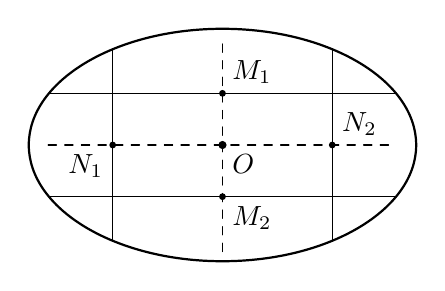
\begin{tikzpicture}[scale=0.82, line cap=round, line join=round]
  % Schematic only: dimensions and directions are not inferred from the source drawing.
  \draw[thick] (0,0) ellipse (3 and 1.8);

  % Two pairs of parallel chords and their midpoints.
  \draw (-2.69,0.8) -- (2.69,0.8);
  \draw (-2.69,-0.8) -- (2.69,-0.8);
  \draw (-1.7,-1.48) -- (-1.7,1.48);
  \draw (1.7,-1.48) -- (1.7,1.48);

  % Lines through the midpoints of each parallel-chord family.
  \draw[dashed] (0,-1.65) -- (0,1.65);
  \draw[dashed] (-2.7,0) -- (2.7,0);

  \fill (0,0.8) circle (1.5pt) node[above right] {$M_1$};
  \fill (0,-0.8) circle (1.5pt) node[below right] {$M_2$};
  \fill (-1.7,0) circle (1.5pt) node[below left] {$N_1$};
  \fill (1.7,0) circle (1.5pt) node[above right] {$N_2$};
  \fill (0,0) circle (1.8pt) node[below right] {$O$};
\end{tikzpicture}
